


\tikzset{every picture/.style={line width=0.75pt}} %set default line width to 0.75pt        

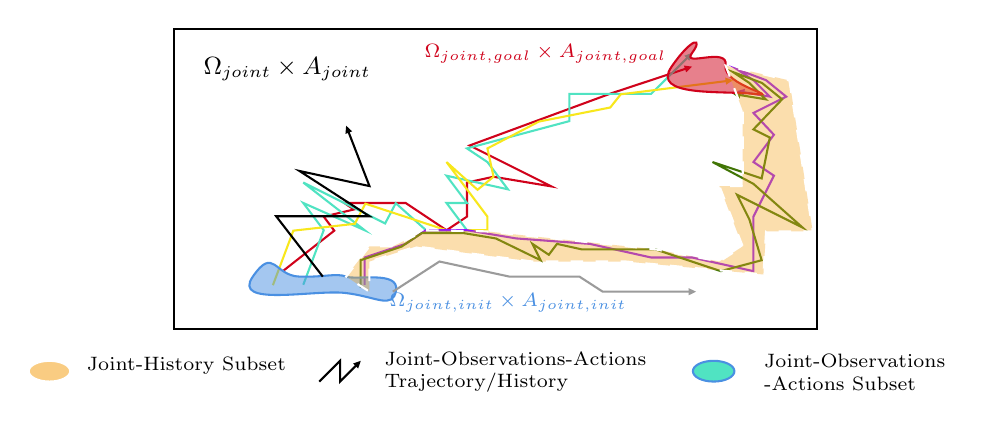
\begin{tikzpicture}[x=0.75pt,y=0.75pt,yscale=-1,xscale=1]
%uncomment if require: \path (0,839); %set diagram left start at 0, and has height of 839

%Shape: Rectangle [id:dp20019810479006872] 
\draw  [fill={rgb, 255:red, 255; green, 255; blue, 255 }  ,fill opacity=1 ] (110,280) -- (420,280) -- (420,424.53) -- (110,424.53) -- cycle ;
%Straight Lines [id:da5726751510023407] 
\draw [color={rgb, 255:red, 208; green, 2; blue, 27 }  ,draw opacity=1 ]   (356.76,299.2) -- (320.56,311.16) -- (252.41,336.26) -- (291.84,355.97) -- (263.95,351.32) -- (251.15,354.1) -- (251.15,370.52) -- (242.82,376.08) -- (241.29,377.09) -- (236.56,373.94) -- (221.58,363.95) -- (192,363.95) -- (196.7,367.09) -- (182.14,370.52) -- (187.22,377.29) -- (162.42,396.8) ;
\draw [shift={(359.6,298.26)}, rotate = 161.71] [fill={rgb, 255:red, 208; green, 2; blue, 27 }  ,fill opacity=1 ][line width=0.08]  [draw opacity=0] (3.57,-1.72) -- (0,0) -- (3.57,1.72) -- cycle    ;
%Straight Lines [id:da03709447257821963] 
\draw [color={rgb, 255:red, 80; green, 227; blue, 194 }  ,draw opacity=1 ]   (357.48,293.81) -- (339.89,311.39) -- (300.45,311.39) -- (300.45,324.53) -- (251.15,337.67) -- (261.01,344.24) -- (270.87,357.38) -- (241.29,350.81) -- (251.15,363.95) -- (241.29,363.95) -- (251.15,377.09) -- (231.44,377.09) -- (216.84,364.08) -- (211.72,373.81) -- (172.28,354.1) -- (201.86,377.09) -- (172.28,363.95) -- (182.14,377.09) -- (172.28,403.37) ;
\draw [shift={(359.6,291.69)}, rotate = 135.01] [fill={rgb, 255:red, 80; green, 227; blue, 194 }  ,fill opacity=1 ][line width=0.08]  [draw opacity=0] (3.57,-1.72) -- (0,0) -- (3.57,1.72) -- cycle    ;
%Straight Lines [id:da5620930288001387] 
\draw [color={rgb, 255:red, 248; green, 231; blue, 28 }  ,draw opacity=1 ]   (376.35,305.2) -- (325.25,311.6) -- (320.17,317.96) -- (285.81,324.74) -- (261.01,337.67) -- (263.95,351.32) -- (256.24,357.59) -- (241.29,344.24) -- (261.01,370.52) -- (261.01,377.09) -- (241.29,377.09) -- (202.21,364.29) -- (197.08,374.01) -- (167.5,377.29) -- (157.64,403.57) ;
\draw [shift={(379.32,304.82)}, rotate = 172.86] [fill={rgb, 255:red, 248; green, 231; blue, 28 }  ,fill opacity=1 ][line width=0.08]  [draw opacity=0] (3.57,-1.72) -- (0,0) -- (3.57,1.72) -- cycle    ;
%Straight Lines [id:da2589856110697837] 
\draw [color={rgb, 255:red, 144; green, 19; blue, 254 }  ,draw opacity=1 ]   (384.25,310.57) -- (397.07,312.71) -- (389.18,304.82) -- (381.29,299.57) -- (395.27,304.82) -- (404.96,312.71) -- (389.18,320.59) -- (399.04,331.1) -- (389.18,344.24) -- (399.04,350.81) -- (389.18,370.52) -- (389.18,396.8) -- (359.6,390.23) -- (339.89,390.23) -- (329.22,387.86) -- (323.58,386.61) -- (315.57,384.83) -- (310.31,383.66) -- (290.52,382.2) -- (274.82,381.03) -- (267.08,379.74) -- (251.15,377.09) -- (231.44,377.09) -- (221.58,383.66) -- (201.86,390.23) -- (201.86,403.37) ;
\draw [shift={(381.29,310.08)}, rotate = 9.46] [fill={rgb, 255:red, 144; green, 19; blue, 254 }  ,fill opacity=1 ][line width=0.08]  [draw opacity=0] (3.57,-1.72) -- (0,0) -- (3.57,1.72) -- cycle    ;
%Straight Lines [id:da048911065410243815] 
\draw [color={rgb, 255:red, 65; green, 117; blue, 5 }  ,draw opacity=1 ]   (382.28,311.89) -- (395.1,314.02) -- (387.21,306.14) -- (379.32,300.88) -- (393.29,306.14) -- (402.98,314.02) -- (389.18,328.48) -- (397.07,332.42) -- (393.13,352.13) -- (369.46,344.24) -- (389.18,354.75) -- (412.84,375.78) -- (381.29,360.01) -- (387.21,371.84) -- (393.13,391.54) -- (373.41,396.8) -- (341.86,386.29) -- (318.2,386.29) -- (306.36,386.29) -- (294.53,383.66) -- (290.59,388.92) -- (282.7,383.66) -- (286.65,391.54) -- (265.11,381.06) -- (249.18,378.41) -- (229.46,378.41) -- (219.6,384.98) -- (199.89,391.54) -- (199.89,404.68) ;
\draw [shift={(379.32,311.39)}, rotate = 9.46] [fill={rgb, 255:red, 65; green, 117; blue, 5 }  ,fill opacity=1 ][line width=0.08]  [draw opacity=0] (3.57,-1.72) -- (0,0) -- (3.57,1.72) -- cycle    ;
%Shape: Polygon Curved [id:ds4136018935395862] 
\draw  [color={rgb, 255:red, 74; green, 144; blue, 226 }  ,draw opacity=1 ][fill={rgb, 255:red, 74; green, 144; blue, 226 }  ,fill opacity=0.5 ] (147.97,399.43) .. controls (158.22,384.65) and (158.23,399.05) .. (170.45,399.43) .. controls (182.67,399.81) and (188.08,397.59) .. (192.93,399.43) .. controls (197.78,401.27) and (218.56,396.47) .. (216.98,406) .. controls (215.4,415.53) and (207.47,408.93) .. (192.28,407.29) .. controls (177.1,405.65) and (137.71,414.21) .. (147.97,399.43) -- cycle ;
%Shape: Polygon Curved [id:ds7172343521236169] 
\draw  [color={rgb, 255:red, 208; green, 2; blue, 27 }  ,draw opacity=1 ][fill={rgb, 255:red, 208; green, 2; blue, 27 }  ,fill opacity=0.5 ] (349.75,298.26) .. controls (360,283.47) and (365.07,284.4) .. (359.6,291.69) .. controls (354.14,298.97) and (377.35,288.24) .. (375.77,297.76) .. controls (374.2,307.29) and (404.36,313.04) .. (389.18,311.39) .. controls (374,309.75) and (339.49,313.04) .. (349.75,298.26) -- cycle ;
%Straight Lines [id:da9382724977616919] 
\draw    (181.69,399.43) -- (159.21,370.35) -- (204.17,370.35) -- (170.45,348.54) -- (204.17,355.81) -- (194.01,329.53) ;
\draw [shift={(192.93,326.73)}, rotate = 68.87] [fill={rgb, 255:red, 0; green, 0; blue, 0 }  ][line width=0.08]  [draw opacity=0] (3.57,-1.72) -- (0,0) -- (3.57,1.72) -- cycle    ;
%Straight Lines [id:da21640651709505887] 
\draw [color={rgb, 255:red, 155; green, 155; blue, 155 }  ,draw opacity=1 ]   (215.41,406.7) -- (237.89,392.16) -- (271.61,399.43) -- (305.33,399.43) -- (316.57,406.7) -- (358.53,406.7) ;
\draw [shift={(361.53,406.7)}, rotate = 180] [fill={rgb, 255:red, 155; green, 155; blue, 155 }  ,fill opacity=1 ][line width=0.08]  [draw opacity=0] (3.57,-1.72) -- (0,0) -- (3.57,1.72) -- cycle    ;
%Shape: Polygon [id:ds6231892522737159] 
\draw  [color={rgb, 255:red, 255; green, 255; blue, 255 }  ,draw opacity=1 ][fill={rgb, 255:red, 245; green, 166; blue, 35 }  ,fill opacity=0.37 ][dash pattern={on 4.5pt off 4.5pt}] (406.49,304.93) -- (417.73,377.62) -- (395.25,377.62) -- (393.97,398.42) -- (327.81,392.16) -- (282.85,392.16) -- (226.65,384.89) -- (204.17,392.16) -- (204.17,406.7) -- (192.93,399.43) -- (204.17,384.89) -- (215.41,384.89) -- (231.44,377.09) -- (260.37,377.62) -- (341.86,386.29) -- (372.77,392.16) -- (384.01,384.89) -- (372.77,355.81) -- (384.01,355.81) -- (384.01,348.54) -- (384.01,319.46) -- (375.77,297.76) -- cycle ;
%Shape: Ellipse [id:dp250499714543976] 
\draw  [color={rgb, 255:red, 74; green, 144; blue, 226 }  ,draw opacity=1 ][fill={rgb, 255:red, 80; green, 227; blue, 194 }  ,fill opacity=1 ] (360,445) .. controls (360,442.24) and (364.48,440) .. (370,440) .. controls (375.52,440) and (380,442.24) .. (380,445) .. controls (380,447.76) and (375.52,450) .. (370,450) .. controls (364.48,450) and (360,447.76) .. (360,445) -- cycle ;
%Straight Lines [id:da8142024352093153] 
\draw [color={rgb, 255:red, 0; green, 0; blue, 0 }  ,draw opacity=1 ]   (197.88,442.12) -- (190,450) -- (190,440) -- (180,450) ;
\draw [shift={(200,440)}, rotate = 135] [fill={rgb, 255:red, 0; green, 0; blue, 0 }  ,fill opacity=1 ][line width=0.08]  [draw opacity=0] (3.57,-1.72) -- (0,0) -- (3.57,1.72) -- cycle    ;
%Shape: Ellipse [id:dp3651678325637011] 
\draw  [color={rgb, 255:red, 255; green, 255; blue, 255 }  ,draw opacity=1 ][fill={rgb, 255:red, 245; green, 166; blue, 35 }  ,fill opacity=0.57 ] (40,445) .. controls (40,442.24) and (44.48,440) .. (50,440) .. controls (55.52,440) and (60,442.24) .. (60,445) .. controls (60,447.76) and (55.52,450) .. (50,450) .. controls (44.48,450) and (40,447.76) .. (40,445) -- cycle ;


% Text Node
\draw (289,292) node  [font=\scriptsize,color={rgb, 255:red, 208; green, 2; blue, 27 }  ,opacity=1 ] [align=left] {$\displaystyle \Omega _{joint,goal} \times A_{joint,goal}$};
% Text Node
\draw (164.5,299.5) node  [font=\small,color={rgb, 255:red, 0; green, 0; blue, 0 }  ,opacity=1 ] [align=left] {$\displaystyle \Omega _{joint} \times A_{joint}$};
% Text Node
\draw (271,412) node  [font=\scriptsize,color={rgb, 255:red, 74; green, 144; blue, 226 }  ,opacity=1 ] [align=left] {$\displaystyle \Omega _{joint,init} \times A_{joint,init}$};
% Text Node
\draw (116,442.5) node  [font=\scriptsize,color={rgb, 255:red, 0; green, 0; blue, 0 }  ,opacity=1 ] [align=left] {Joint-History Subset};
% Text Node
\draw (274.5,445.5) node  [font=\scriptsize,color={rgb, 255:red, 0; green, 0; blue, 0 }  ,opacity=1 ] [align=left] {Joint-Observations-Actions\\Trajectory/History};
% Text Node
\draw (438,445.5) node  [font=\scriptsize,color={rgb, 255:red, 0; green, 0; blue, 0 }  ,opacity=1 ] [align=left] {Joint-Observations\\\mbox{-}Actions Subset};


\end{tikzpicture}